\documentclass[border=10pt]{standalone}

\usepackage{tikz}
\usepackage{tikzsymbols}
\usetikzlibrary{calc,patterns,shapes.geometric}

\def\centerarc[#1](#2)(#3:#4:#5){\draw[#1] ($(#2)+({#5*cos(#3)},{#5*sin(#3)})$) arc (#3:#4:#5);}

\begin{document}
	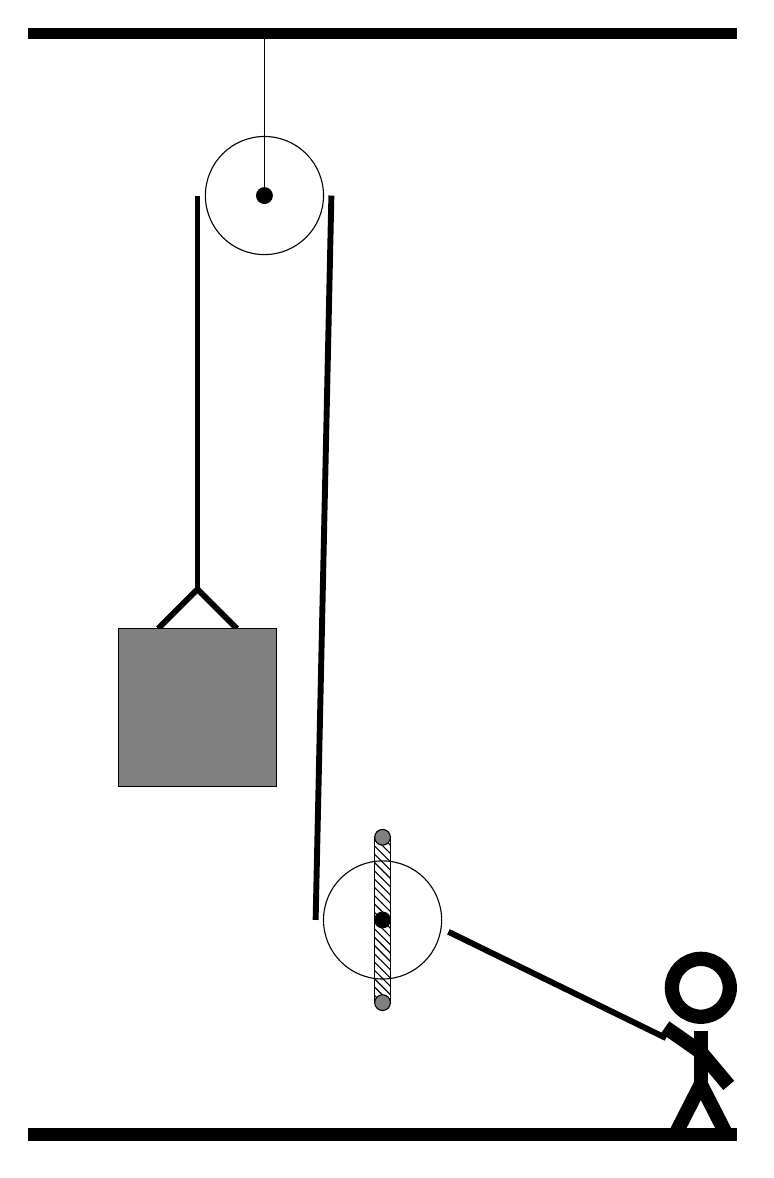
\begin{tikzpicture}
		%%%%% START %%%%%
		\draw[fill=black] (-2, 14) rectangle (7, 14.125);
		
		\draw (1, 12) circle (0.75);
		\draw[fill=black] (1, 12) circle (0.1);
		\draw (1, 14) -- (1, 12);
		
		\draw[fill=white](2.5, 2.8) circle (0.75);
		\draw[fill=black] (2.5, 2.8) circle (0.1);
		\draw[pattern=north west lines, pattern color=black] (2.4, 3.85) rectangle (2.6, 1.75);
		\draw[fill=black!50] (2.5, 3.85) circle (0.1);
		\draw[fill=black!50] (2.5, 1.75) circle (0.1);
		
		\draw[line width=0.75mm] (-0.35, 6.5) -- (0.15, 7.0) -- (0.65, 6.5);
		\draw[fill=black!50] (-0.85, 6.5) rectangle (1.15, 4.5);
		
		\draw[line width=0.75mm] (0.15, 12) -- (0.15, 7.0);
		\centerarc[line width=0.75mm](1, 12)(0:180:0.85);
		\draw[line width=0.75mm](1.85, 12) -- (1.65, 2.8);
		\centerarc[line width=0.75mm](2.5, 2.8)(180:270:0.85);
		\draw[line width=0.75mm](3.336, 2.65) -- (6.1, 1.3);
		
		\node at (6.5, 1.2) {\Strichmaxerl[10][-35][-50]};
		
		\draw[fill=black] (-2, 0) rectangle (7, 0.15);
		%%%%% END %%%%%
	\end{tikzpicture}
\end{document}